\documentclass[a4paper,12pt]{article} 
\sloppy

% report, book

% Рисунки
\usepackage{graphicx}
\DeclareGraphicsExtensions{.pdf,.png,.jpg}
\usepackage{wrapfig}
% Гиперссылки
\usepackage{hyperref}
\usepackage[rgb]{xcolor}
\hypersetup{
    colorlinks=true,
	urlcolor=blue,
    unicode=true
}

%  Русский язык

\usepackage[T2A]{fontenc} % кодировка
\usepackage[utf8]{inputenc} % кодировка исходного текста
\usepackage[english,russian]{babel}	% локализация и переносы
\usepackage {indentfirst} % отступ
\usepackage[left=2.5cm,right=2.5cm,
    top=2cm,bottom=2cm,bindingoffset=0cm]{geometry}

% Кавычки
\usepackage {csquotes}
\DeclareQuoteStyle{russian}
    {\guillemotleft}{\guillemotright}[0.025em]
    {\quotedblbase}{\textquotedblleft}
\ExecuteQuoteOptions{style=russian}

% Код
\usepackage {listings}
\lstset{tabsize=2,
    breaklines,
    columns=fullflexible,
    flexiblecolumns,
    numbers=left,
    numberstyle={\footnotesize},
    extendedchars}


% Математика
\usepackage{amsmath,amsfonts,amssymb,amsthm,mathtools} 
\usepackage{biblatex}
\addbibresource{biblio.bib}



\usepackage{wasysym}
\begin{document} 
\title{Adversarial атака на людей.}
\author{Андрей Поповкин}
\maketitle

\section{Введение}
Модели машинного обучения уязвимы к так называемым adversarial examples: небольшим изменениям входных данных, приводящим к тому, что модели совершают ошибки, порой абсолютно неадекватные с точки зрения человека, как например в примере с пандой, распознающейся как гиббон \ref{fig:panda}. В данном случае изменение входного изображения было подобрано специально для атаки конкретной модели. Однако существуют исследования, демонстрирующие возможность и способы создания изображений, вводящих в заблуждение сразу множество моделей, в том числе с неизвестной архитектурой. Подобный подход возможно использовать для создания примеров, вводящих в заблуждение не только модели машинного обучения, но и людей.

\begin{figure}[h]
\centering
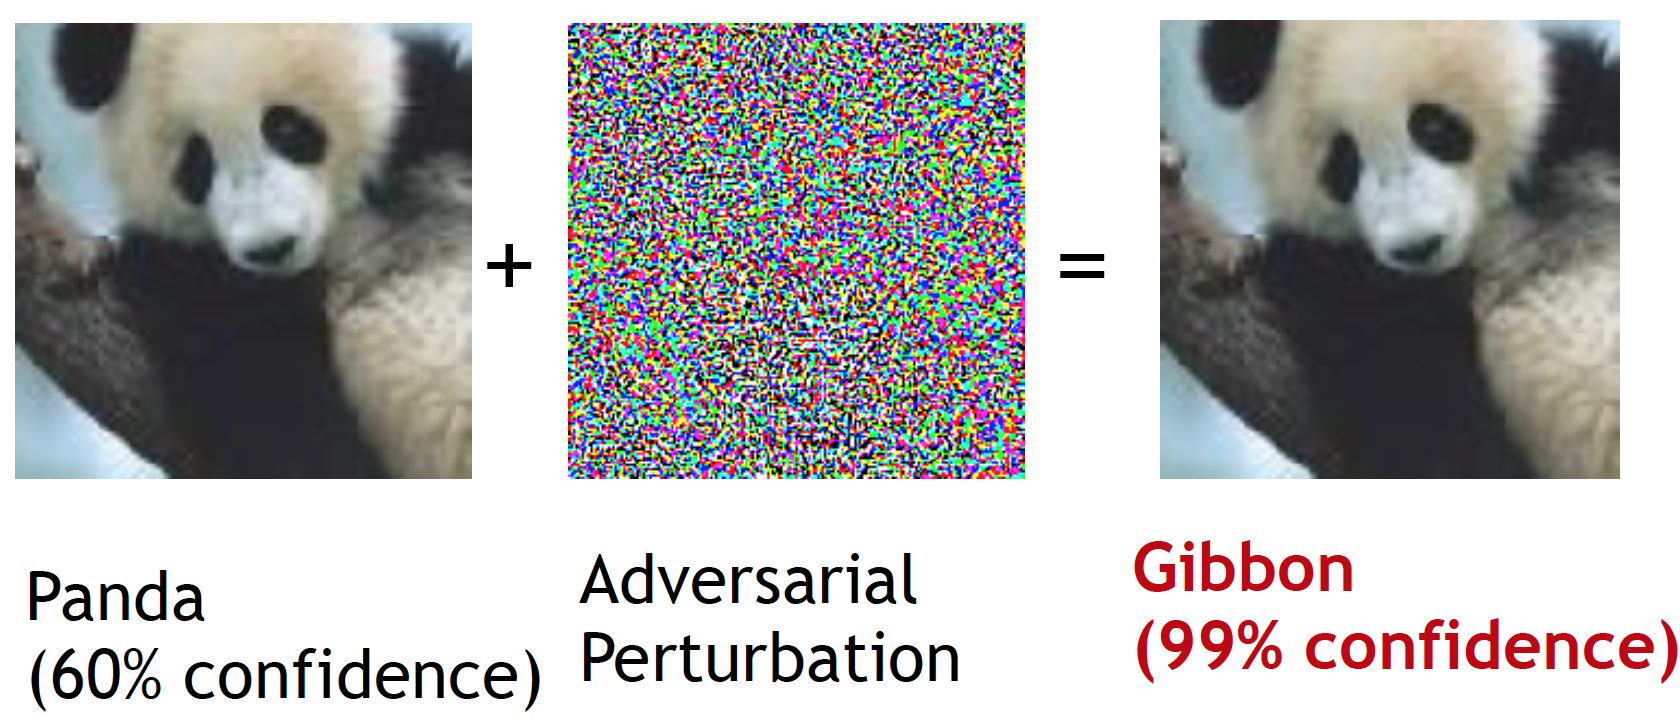
\includegraphics[width=0.7\linewidth]{panda.png}
\caption{Adversarial example, обманывающий модель классификации.}
\label{fig:panda}
\end{figure}

\section{Определение}
В оригинальной статье про adversarial examples дается следующее определение (вольный перевод на русский):
<<Входные данные для модели машинного обучения, намеренно созданные злоумышленником для того, чтобы модель совершила ошибку.>> В области компьютерного зрения, под adversarial example, обычно понимают слабое изменение изображения, заставляющее модель классификации изменить предсказываемый класс.

Чтобы внести ясность, нужно зафиксировать пару уточнений к определению:
\begin{enumerate}
    \item Adversarial examples создаются с целью вызвать ошибку в классификации. Но не для того, чтобы вызвать классификацию, отличную от человеческой. В противном случае, создать adversarial example для человека невозможно по определению.
    \item Adversarial examples НЕ обязательно неразличимы человеком \ref{fig:cat}.
\end{enumerate}

\begin{figure}[h]
\centering
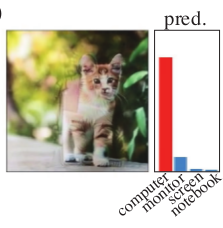
\includegraphics[width=0.3\linewidth]{cat.png}
\caption{Adversarial example, заметный человеку. Более того, человек способен понять, почему модель предсказывает класс <<компьютер>>, т.к. изображение обладает понятными человеку <<фичами>> компьютера.}
\label{fig:cat}
\end{figure}

\section{Эксперимент}
Участнику эксперимента, фокусирующему взгляд в центре экрана, демонстрировалось изображение на протяжении приблизительно одной двадцатой секунды (на границе различимости), после которой демонстрировался набор контрастных шумов. После этого предлагалось определить изображение к одному из двух классов: кошки-собаки, змеи-пауки или капуста-брокколи.

Такие жесткие ограничения по времени диктуются тем, что зрительная кора человеческого мозга устроена гораздо сложнее однонаправленного вычислительного графа сверточных нейронных сетей. И стимуляция на коротком временном промежутке призвана уменьшить врияние обратных и реккурентных связей зрительной коры. Кроме того, человеческий глаз стремится исследовать наблюдаемую сцену, например, посредством саккад, с течением времени получая все больше и больше деталей.

Тем не менее, существуют исследования, проводящие параллели между устройством и генерируемыми сигналами в сверточных слоях нейронных сетей и сигналами, генерируемыми глубокими слоями зрительной коры, что дает надежды на схожесть способов обработки зрительной информации, тем большую, если исключить существенные различия, указанные выше.

\section{Изображения, использованные для эксперимента}
Эксперимент содержал в себе несколько групп изображений: 
\begin{enumerate}
    \item Исходные изображения из ImageNet, необходимые, чтобы получить оценку на точность классификации человеком в сложных условиях эксперимента.
    \item Adversarial examples, заставляющие ансамбль моделей машинного обучения ошибаться в пользу парного класса.
    \item Изображения, с добавлением того же возмущения, что и в adversarial examples, но отраженного по вертикали. Такие изображения должны терять способность вводить в заблуждение, однако статистически сохраняют возмущение изображения, приводящее к ухудшению его качества и, как следствие, влияющее на точность классификации человеком.
    \item Изображения, не принадлежащие изучаемым классам, часть которых была обработана, как adversarial example к одному из классов, предлагаемых в качестве ответа. Эта группа имеет целью выяснить, можно ли вызвать среди ответов преобладание одного неверного класса над другим.
\end{enumerate}

\section{Подготовка adversarial examples}
Для достижения лучшего эффекта adversarial examples генерировались при помощи blackbox оптимизации, максимизируя ошибку \ref{loss} ансамбля моделей~--- распространенный способ получения примеров, применимых к множеству заранее не известных моделей.

Таким образом, задача генерации следующая: имея изображение $X$ и целевой ошибочный класс $y_{target}$, получить изображение $X_{adv}$, такое что:
\begin{equation}
\label{loss}
    \begin{cases}
    \log(P_{\theta} (y_{target} | X_{adv} )) \overset{\theta}{\rightarrow} min\\
    ||X_{adv} - X||_{\inf} = \epsilon
    \end{cases}
\end{equation}

Эпсилон выбиралось небольшим, чтобы избежать реального изменения класса изображения, но и достаточным для получения устойчивых ошибок классификации.

Кроме того, изображения были предобработанны с учетом особенностей человеческого восприятия изображений. В первую очередь~--- неоднородности сетчатки, дающей более резкое изображение в центре фокусировки и размытое по краям. 

\section{Результаты}

\begin{figure}[h]
\centering
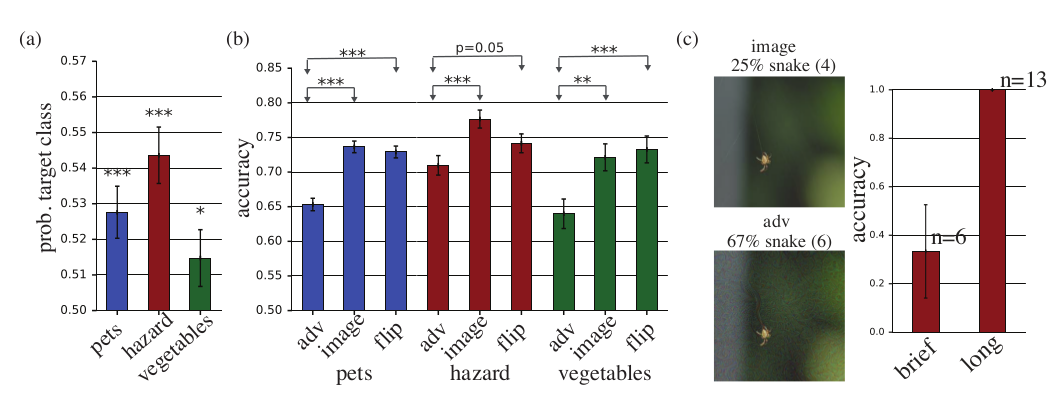
\includegraphics[width=0.99\linewidth]{results.png}
\caption{Результаты эксперимента: (a) вероятность выбора целевого класса в задаче выбора между двумя неправильными классами; (b) точность классификации разных групп изображений; (с) точность классификации конкретного adversarial example в эксперименте и email опросе. Доверительные интервалы~--- стандартное отклонение, количество звезд отвечает за уровень значимости теста на присутствие различия. *:~$p < 0.05$; **:~$p < 0.01$; ***:~$p < 0.001$.}
\label{fig:results}
\end{figure}

В итоге авторам удалось провести очень качественный, с методической точки зрения, эксперимент, показывающий, что при специфичных условиях наблюдения, возможно создание adversarial examples, вводящих в заблуждение человека. Более того, даже в случае отсутствия возможности дать правильный ответ, специальная обработка изображения приводит к смещению ответов в сторону целевого класса. Особенно значительный эффект достигается в случае с классами <<опасностей>>: змеи и пауки, что достаточно естественно с эволюционной точки зрения. Очень значительное различие в точности классификации наблюдается и в непосредственно целевом эксперименте. Модифицированные изображения классифицируются с почти на 10\% меньшей точностью. Кроме того, было показанно, что специфичные условия эксперимента очень существенны, т.е. при неограниченном времени изучения аугментированного изображения, точность его классификации приближается к абсолютной.

\section{Итоги}

Adversarial examples интересны в первую очередь с точки зрения безопасности. Огромные усилия направленны на производство антиспуфинг защиты, например, для систем аутентификации мобильных устройств. И полученные результаты показывают, что <<эталонная>> система распознавания образов человека сама по себе уязвима к атакам, правда в достаточно специфичных условиях. Это важные данные, как для безопасности: по всей видимости, архитектуры на основе сверток по своей природе уязвимы перед уже известными способами атаки. Так и с точки зрения нейробиологии, демонстрируя существенность обратных и реккурентных связей зрительной коры для конкретной задачи классификации.

\printbibliography[heading=bibintoc]
\end{document}